\chapter{Mayer Vietoris \& Persistent Homology}
In the chapter we demonstrated how to compute homology using the \mvb{} or equivalently the \mv spectral sequence. In this chapter we expand on this, to show how we can adapt these procedures to computing persistent homology. To do this, we will first observe that there exists a filtration on the blowup complex which produces identical persistent homology to a filtration on the base space. Then we will show how we can use the structure of the blowup complex to extract some parallelism, while still computing the correct result. In order to acheive this, we need to characterize when two filtrations will produce the same persistent homology. 
\begin{theorem}{Persistence Equivalence Theorem}
    Given two filtrations $L_0 \subseteq \ldots \subseteq L_n$ and
    $K_0 \subseteq \ldots \subseteq K_n$, the induced sequences of homology
    groups produce the same persistence pairs,
    if the there are vertical isomorphisms $H(K_i) \to H(L_i)$ that makes the entire diagram commute.
\[
\begin{tikzcd}[row sep=large, column sep=small]
    H_*(K_1) \arrow{r}\arrow{d} & \ldots \arrow{r} & H_*(K_i)  \arrow{r}\arrow{d} & \ldots \arrow{r} & H(K_n) \arrow{d} \\
    H_*(L_1) \arrow{r} & \ldots \arrow{r} & H_*(L_i)  \arrow{r} & \ldots \arrow{r} & H(L_n) \\
\end{tikzcd}
\]
\end{theorem}
\begin{proof}
See Zomorodian and Carlsson~\cite{zc-cph-05}
\end{proof}
Now we need to produce a filtration on the blowup complex to use as a row of one of these filtrations. To do this, observe that if $\{K_i\}$ is a filtration on the base space, and $\C =\{ \C_i \}$ is a cover of $K_n$, that by restriction, this provides a cover of all the spaces in the filtration. Now, each of these covers is closed, and there is an associated blowup complex. It is easy to see that these blowup complexes also form a filtration, with the same number of terms as the original space. Recall that the projection map, $\pi: \K_i^\C \to \K_i$, is also a homotopy equivalence, and so the map $\pi^*: H(\K^\C) \to H(K)$, induced on homology modules, is an isomorphism. Also the map $\pi$ clearly commutes with inclusions, by construction, so  the persistence equivalence theorem applies. We now explain this filtration again, using partial orders.

Recall that we computed the homology of the blowup complex, by computing the persistent homology of a two step filtration, which ordered product cells $\sigma \otimes \tau \leq \sigma'  \otimes \tau'$ where $\sigma,\sigma' \in \K$ and $\tau, \tau' \in N$. It is not hard to see that if one simply reverses this comparison, and first compares the base complex term, breaking ties by the factor in the nerve, that this partial order is equivalent to the filtration defined in the previous statement. However, these two filtrations have a bit more in common. We state the following lemma without proof.
\begin{lemma}
Denote the two filtrations $\leq_N$ and $\leq_K$ respectively
Fix any $\tau \in N$, if $\alpha, \beta \in K$ such that $\alpha \times \tau, \beta \times \tau \in \K^\C$ then $\alpha \times \tau \leq_K \beta \times \tau$ if and only if $\alpha \times \tau \leq_N \beta \times \tau$
\end{lemma}

This implies that the following reduction algorithm would be correct.:
\begin{enumerate}
\item First, reduce all submatrices corresponding to product cells with a fixed nerve factor in parallel. 
\item Further reduce the matrix in the correct $\leq_K$ filtration order.
\end{enumerate}
The goal will be to begin the procedure the same way as we did in the previous chapter, first reduce the columns, corresponding to the boundaries of the cells $_ \times \tau$ for fixed $\tau$ independently, and then merge these results together. In particular, the important observation, is that each of these subsets of columns, are by themselves, respecting the filtration order. Therefore if we naively just reduced the remaining matrix sequentially, this would result in the correct algorithm. However, this would be inefficient.

The trouble here is that as stated, performing only column operations, we have no control over the fill in of the resulting matrix. However, we may now take advantage of the sparsity pattern to reduce the space complexity. Over each submatrix corresponding to a vertex in the nerve, we may perform row operations in a specific order signficantly reduce the fill in. The algorithm $\proc{Sparsify}$ is used on the submatrix whose rows fall in the disjoint union.

\begin{figure}
\begin{codebox}
$\Procname{\proc{Sparsify}(R)}$
\li $P = R$, $S = I$
\li    \For{rows $\row{P}{i}$ of $P$ from bottom up} 
\li \Do \If{$P[i,j]$ is not zero}
\li            \For{non-zero entries $P[i', j]$ in $\col{P}{j}$, with $i' \neq i$}
\li		  $\row{P}{i'} = \row{P}{i'} - \row{P}{i}$  \Comment{zero out the entry $P[i',j]$}
\li		  $\col{S}{i} = \col{S}{i} + \col{S}{i'}$
            \End
        \End
    \End
\end{codebox}
\caption{Column sparsification algorithm.}
\label{alg:sparsify}
\end{figure}

After applying $\proc{Sparsify}$ we make use of the algorithm $\proc{Cascade}$ to finish the reduction. This is similar to the standard algorithm, in that columns are still added in order, but, when a pivot is found, we perform row operations to sparsify the final column.

\begin{figure}
\begin{codebox}
$\Procname{\proc{Cascade}(T)}$
\li    \For{rows $\row{T}{i}$, from bottom up}
\li    \Do
\li         $J$ = columns with the lowest non-zero entry in row $\row{T}{i}$
\li $j = \min J$
\li \For{$j' \in J, j' > j$}
 \li \Do  subtract $\col{T}{j}$ from $\col{T}{j'}$
\End
\li \For{$i' < i$ with $T[i,j] \neq 0$}
\li \Do  subtract $\row{T}{i}$ from $\row{T}{i'}$     \Comment{zero out all but the lowest entry of column $\col{T}{j}$}
        \End
    \End
\end{codebox}
\caption{Cascade algorithm for the reduction of the matrix $T$ with ultra-sparse columns.}
\label{alg:cascade}
\end{figure}

We can now state the following result:

\begin{theorem}
    \label{thm:complexity}
    $\alg{Cascade}(T)$ algorithm reduces the matrix $T$ with $n$ ultra-sparse and
    $m$ dense columns in time $O(n^2 m)$, while keeping its size $O(nm)$.
\end{theorem}
\begin{proof}
    The initial number of nonzero elements in the matrix $T$ is in $O{(n + m) m + n} = O(nm)$.
     By using row operations applied to column $j$ the number of dense columns never increases. So the
     space used during the cascade remains $O(nm)$.

    It takes $O(n+m)$ time to add two dense columns, or to add a dense
    column to a sparse column. How many such operations are there?
    At most $m$ per row. There are $n+m$ rows, for a total of
    $O((n+m)^2 m) = O(n^2 m)$ operations.
\end{proof}

So far we have considered the case of a single cover of the domain, a collection
of simplicial complexes $K = \{ K^i \}_I$ with domain $K = \bigcup \C$. But in many
applications, it is natural to build a hierarchy of such covers. 
For example, if the domain $K$ triangulates a cube or a flat torus, both exceedingly common scenarios for
simulation data, one can build a refinement of covers following an oct-tree
partition of the cube. The closures of the sub complexes identified by the cubes at each level of the oct-tree 
become the cover sets. It is natural to utilize spatial locality in a covering to try and perform less communication.
In the next section we explore how to utilize this hierarchy in the algorithm.

\section{Hierarchy}
\label{sec:hierarchy}
Suppose that we have a nested collection of
covers $\C_0, \C_1, \ldots$, such that $K = \bigcup \C_0 = \bigcup \C_1 = \ldots$
and every cover set $L^i \in \C_a$ is contained in exactly one cover set
$K^j \in \C_{a-1}$, $L^i \subseteq K^j$

One may reduce the boundary matrixes restricted to local groups in this hierarchy,
extending the amount of useful work a processor can do. This also limits how
many dense columns a single processor has to handle at once.
%
Consider an oct-tree with $p = 8^k$ processors. At the $k$-th level in the
tree, we end up with $p$ cubes and an intersection of size $m = 3 \cdot 2^k \cdot c$,
where $c$ is the number of simplices in a side of the cube. By merging the cubes in pairs, e.g,  higher level
in the hierarchy after each merge, $m$ never exceeds $c$, the size of the
initial cut that splits the domain into two.

Consider the structure of the boundary matrix for two consecutive levels in the
cover, illustrated in Figure~\ref{fig:hierarchy}. Suppose at level $i+1$ the
cover consists of four sets, $\C_{i+1} = \{ K^1, K^2, K^3, K^4 \}$, and at level
$i$ the cover consists of two sets $\C_i = \{ K^1 \cup K^2, K^3 \cup K^4 \}$.
%
The procedures $\proc{Sparsify}$ and $\proc{Cascade}$ would operate independently
on the matrices $D^1, D^2, D^3,$ and $D^4$ (on four different processors). The first
two results would then be combined by first performing row updates on the matrices $Q^1$ and
$Q^2$, then reordering the matrix and reducing it using the {\bf Cascade}
algorithm.

The second pair of results would be combined similarly.
The two combined matrices contain the same information as the reduced boundary
matrices $R^{12}$ and $R^{34}$ for the cover sets $K^1 \cup K^2$
and $K^3 \cup K^4$ at level $i$. We could proceed with the algorithm at level
$i$, with one caveat: the higher rows (the second to last column in the figure)
involved in the combination did not get updated during the execution of {\bf
Sparsify} and {\bf Cascade} algorithms. The fix is straight-forward: when
processing any given level of the cover, we perform the row operations on the
full rows, rather than on their restriction to the given level.
The only information necessary to construct such rows is knowing which sets of
the cover contain any given simplex.

\begin{figure}
    \centering
    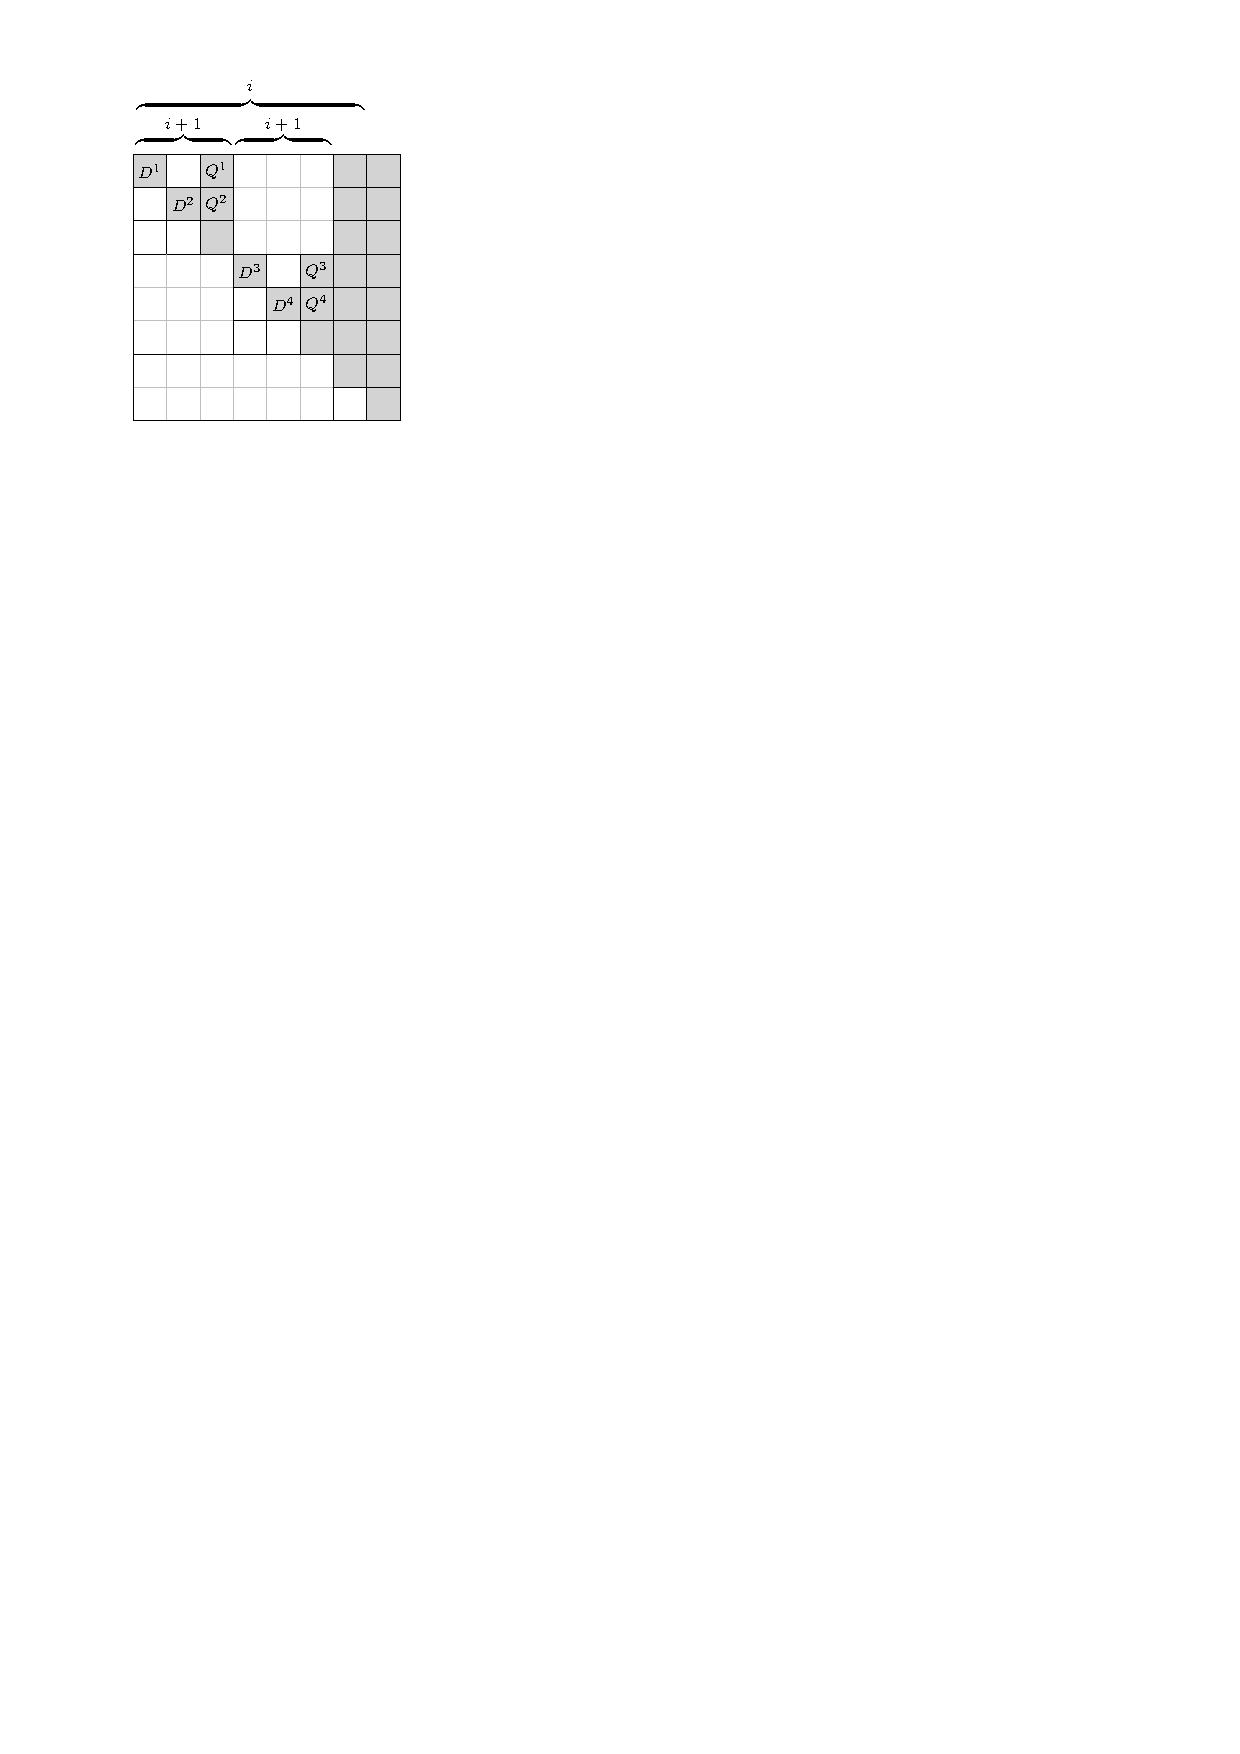
\includegraphics{figs/hierarchy}
    %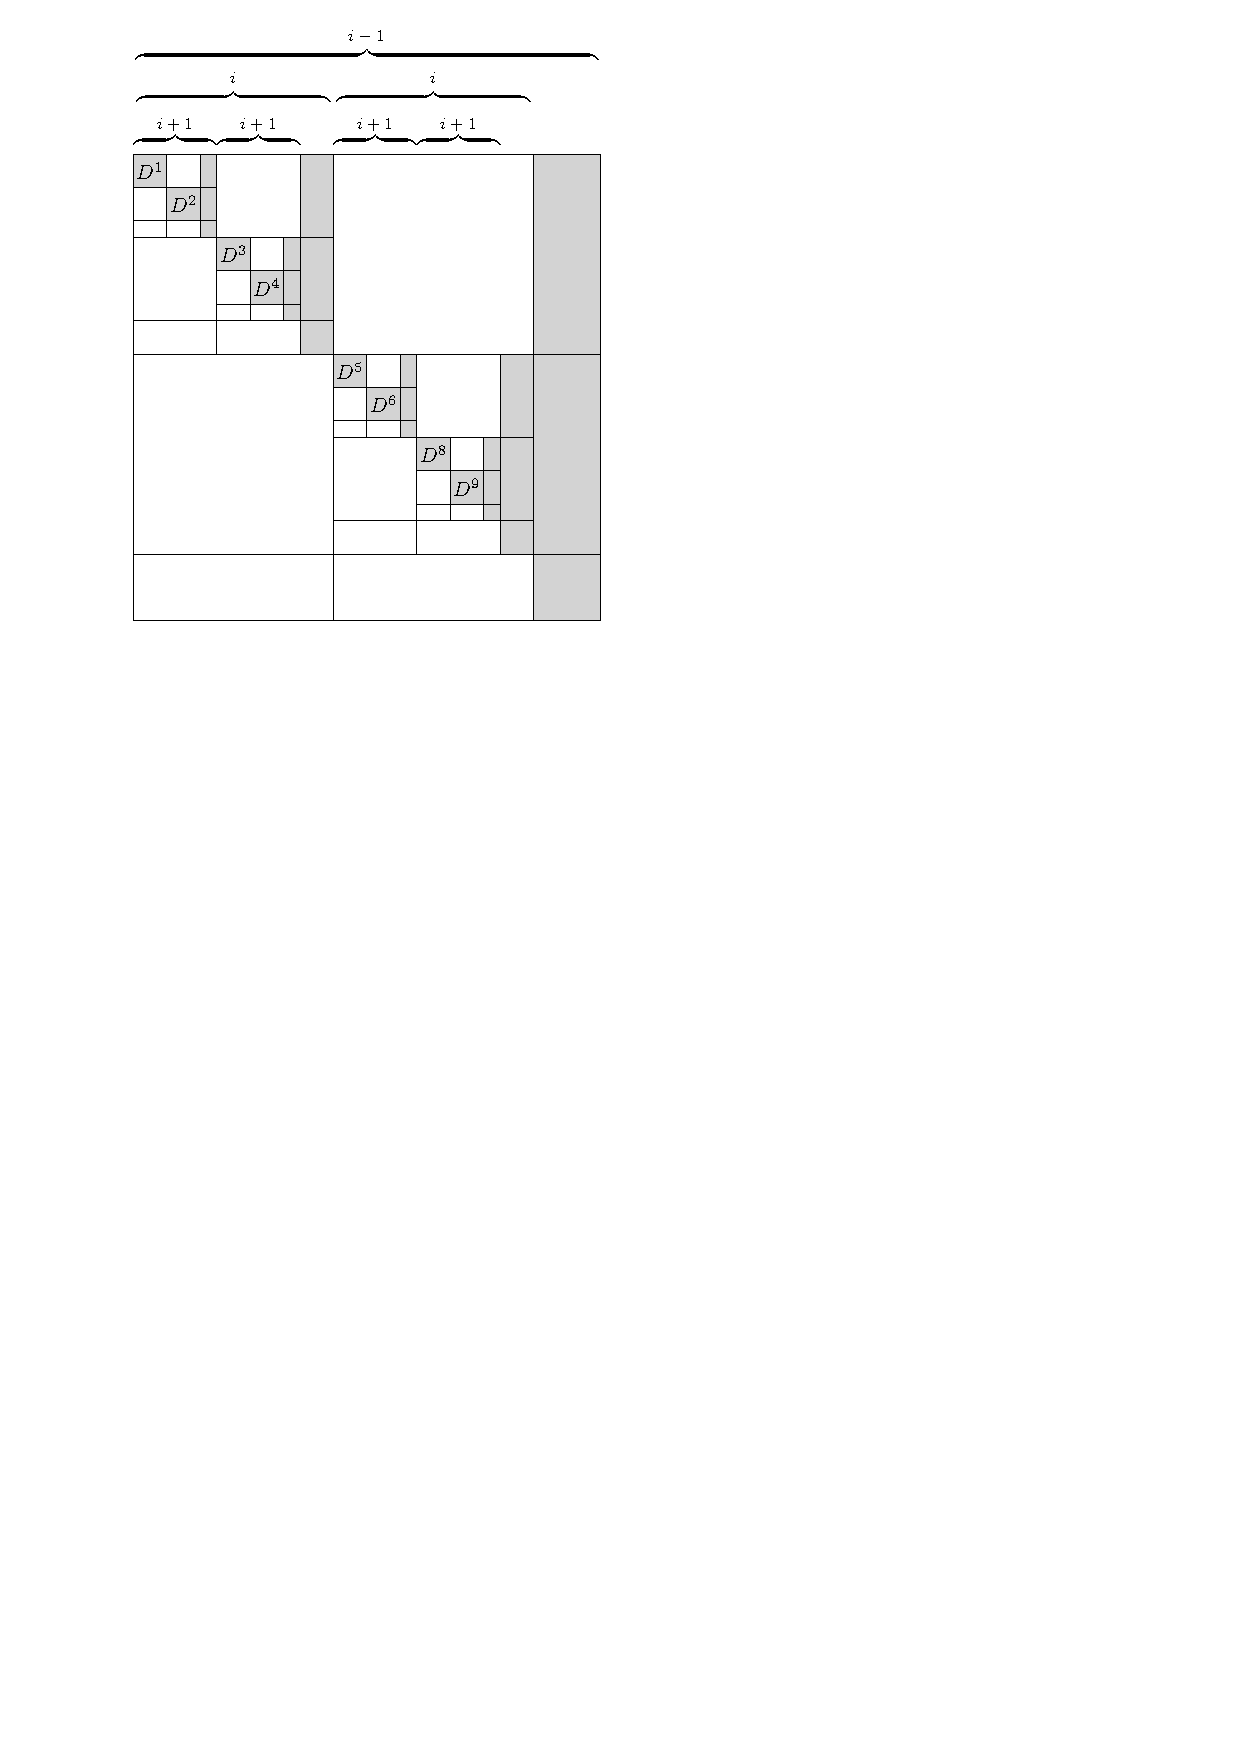
\includegraphics[width=.46\textwidth]{figs/boundary-hierarchy}
    \caption{The structure of the boundary matrix for three consecutive levels of
             the hierarchy.}
    \label{fig:hierarchy}
\end{figure}

\section{Experiments}
\label{sec:experiments}

We have implemented the described algorithm on top of MPI, and ran a strong
scaling experiment on Edison supercomputer at the National Energy Research
Scientific Computing Center (NERSC). Edison is a Cray XC30 system; its
individual compute nodes have 24 Intel `Ivy Bridge' processor cores, at 2.4 GHz,
with 64KB and 256KB of L1 and L2 cache, respectively; the 24 cores share 64GB of RAM.

Our input is a snapshot of a combustion simulation, a $256^2 \times 512$ scalar
field.
%of density \Remark{of what} during a burning of methane.
The input simplicial complex is a Freudenthal triangulation of the grid,
with $\sim 870 \cdot 10^6$ simplices. It is covered hierarchically via an
oct-tree.

Figure~\ref{fig:times} and Table~\ref{tbl:times} summarize the running times
(wallclock as reported by the PBS job resource manager).
Going from 8 to 32 processes we see a near
perfect scaling, with another improvement by a factor of $\sim 1.5$ going from
32 to 64 processes. But then the returns diminish rapidly. The behavior is not
surprising: past 64 processes the binary reduction used to merge
different cover sets is top-heavy, i.e., it's dominated by the merge of the
information from the final two sets. As a result, adding more processes only
speeds up the initial computation, which is already plenty fast.

\pgfplotstableread{data/plt07895.dat}\pltCombustionMed

\begin{figure}
    \centering
    \begin{tikzpicture}
    \begin{axis}[
                    %ybar,
                    %xtick=data,
                    ymode=log,
                    %log basis y=2,
                    tick align=inside,
                    %ymax=100,
                    ymin=580,
                    symbolic x coords={8,16,32,64,128,256,512},
                    height=3in,
                    width=.5\textwidth,
                    xlabel={Number of processes},
                    ylabel={Seconds},
                ]
        \addlegendentry{\hspace{.3in} Persistence ($256^2 \times 512$):}
        \addplot+[] table[x=proc,y=time]
                  {\pltCombustionMed};
        \addlegendentry{\hspace{.3in}Perfect scaling:}
        %\addplot+[dashed, red, mark=none] table[x=proc,y=perfect]
        %          {\pltCombustionMed};
        \addplot+[dashed, red, mark=none] coordinates
                  {
                      (8,  4096)
                      (16, 2048)
                      (32, 1024)
                      (64, 512)
                  };
    \end{axis}
    \end{tikzpicture}

    \caption{Times to compute persistence diagram for the $256^2 \times 512$
             combustion data set. The measurements are in Table~\ref{tbl:times}.}
    \label{fig:times}
\end{figure}

\begin{table}
    \centering
    \pgfplotstabletypeset
    [
        every head row/.style={
            before row={
                \toprule
            },
            after row=\midrule,
        },
        columns={proc, time},
        columns/proc/.style         ={column name=processors, int detect, column type={r}},
        columns/time/.style         ={column name=seconds, fixed, column type={|r}},
    ]
    {\pltCombustionMed}
    \caption{Times to compute persistence diagram for the $256^2 \times 512$
             combustion data set. The data is presented visually in
             Figure~\ref{fig:times}.}
    \label{tbl:times}
\end{table}

We have tried our code on larger data sets, but ran out of memory during the
final stages of the merge reduction. Although the $(n+m)$ term in the space analysis of the
\alg{Cascade} algorithm is a gross worst-case overestimate, the growth of this
term does follow the growth of $n$, the size of the domain, in many practical
examples. So our technique does not solve the memory limitations of the
persistence algorithm for large data sets covered by many relatively small cover sets. This is
intuitive, as the Mayer Vietoris principle is most effective when we can cover a space by large open sets, which do not
have relatively deep intersections. 

Despite the limitations of these new reduction techniques, we believe our theoretical
results have a place as building blocks of a practical parallel persistence algorithm.

It would be fruitful to understand the relationship of our algorithm
to various practical optimizations~\cite{bkr-cccph-13}. 
Unexpectedly to us, the original optimization~\cite{elz-tps-02} that removes negative
simplices from the columns of the matrix $R$ cannot be used in our context.
The reason is that a simplex that is
negative in the filtration of a cover subcomplex $K^i$ may be positive in the
filtration of the entire space $K$.
On the other hand, if a simplex creates a cycle in the filtration of $K^i$
(i.e., it is positive), it must be positive in the filtration of the entire $K$.
Thus the clearing optimization of Chen and Kerber~\cite{bkr-cccph-13}
is readily applicable.

More along those lines, an interesting promising research direction is
combining the techniques outline here for reducing the disjoint union, with out of order optimizations that one can use when
employing the spectral sequence algorithm~\cite{bkr-cccph-13}.

One could initially distribute the data with respect to the disjoint union of an open cover:
often such a distribution is either very cheap to compute, or entirely
free in the cases when the data is supplied already decomposed directly from a simulation code,
or for efficiency reasons it is stored decomposed. The part of our algorithm which processes
the disjoint union scales perfectly. Then, when combining the individual results, one
could redistribute the remaining matrix, the input to the $\alg{Cascade}$
algorithm, with respect to the diagonal block partition of the spectral sequence
algorithm. This way we could limit the space needed on any given processor.
